\documentclass{sigchi}

% Use this command to override the default ACM copyright statement
% (e.g. for preprints).  Consult the conference website for the
% camera-ready copyright statement.


%% EXAMPLE BEGIN -- HOW TO OVERRIDE THE DEFAULT COPYRIGHT STRIP -- (July 22, 2013 - Paul Baumann)
% \toappear{Permission to make digital or hard copies of all or part of this work for personal or classroom use is      granted without fee provided that copies are not made or distributed for profit or commercial advantage and that copies bear this notice and the full citation on the first page. Copyrights for components of this work owned by others than ACM must be honored. Abstracting with credit is permitted. To copy otherwise, or republish, to post on servers or to redistribute to lists, requires prior specific permission and/or a fee. Request permissions from permissions@acm.org. \\
% {\emph{CHI'14}}, April 26--May 1, 2014, Toronto, Canada. \\
% Copyright \copyright~2014 ACM ISBN/14/04...\$15.00. \\
% DOI string from ACM form confirmation}
%% EXAMPLE END -- HOW TO OVERRIDE THE DEFAULT COPYRIGHT STRIP -- (July 22, 2013 - Paul Baumann)


% Arabic page numbers for submission.  Remove this line to eliminate
% page numbers for the camera ready copy 

%\pagenumbering{arabic}

% Load basic packages
\usepackage{balance}  % to better equalize the last page
\usepackage{graphics} % for EPS, load graphicx instead 
%\usepackage[T1]{fontenc}
\usepackage{txfonts}
\usepackage{times}    % comment if you want LaTeX's default font
\usepackage[pdftex]{hyperref}
% \usepackage{url}      % llt: nicely formatted URLs
\usepackage{color}
\usepackage{textcomp}
\usepackage{booktabs}
\usepackage{ccicons}
\usepackage{todonotes}



% My packages
\usepackage{dcolumn}
\usepackage{multirow}
\newcolumntype{d}{D{.}{.}{4.0}}
\newcolumntype{s}{D{.}{.}{1.4}}
\usepackage{arydshln}
\usepackage{enumitem}


% llt: Define a global style for URLs, rather that the default one
\makeatletter
\def\url@leostyle{%
  \@ifundefined{selectfont}{\def\UrlFont{\sf}}{\def\UrlFont{\small\bf\ttfamily}}}
\makeatother
\urlstyle{leo}

% To make various LaTeX processors do the right thing with page size.
\def\pprw{8.5in}
\def\pprh{11in}
\special{papersize=\pprw,\pprh}
\setlength{\paperwidth}{\pprw}
\setlength{\paperheight}{\pprh}
\setlength{\pdfpagewidth}{\pprw}
\setlength{\pdfpageheight}{\pprh}

% Make sure hyperref comes last of your loaded packages, to give it a
% fighting chance of not being over-written, since its job is to
% redefine many LaTeX commands.
\definecolor{linkColor}{RGB}{6,125,233}
\hypersetup{%
  pdftitle={SIGCHI Conference Proceedings Format},
  pdfauthor={LaTeX},
  pdfkeywords={SIGCHI, proceedings, archival format},
  bookmarksnumbered,
  pdfstartview={FitH},
  colorlinks,
  citecolor=black,
  filecolor=black,
  linkcolor=black,
  urlcolor=linkColor,
  breaklinks=true,
}

% create a shortcut to typeset table headings
% \newcommand\tabhead[1]{\small\textbf{#1}}

% End of preamble. Here it comes the document.
\begin{document}

\title{How One Microtask Affects Another}

\numberofauthors{3}
\author{%
  \alignauthor{
	Edward Newell \\
    \affaddr{School of Computer Science, McGill University}\\
    \affaddr{3480 University Street, Room 318, Montreal, Qu\'ebec,
	  Canada, H3A 2A7
	}\\
	\email{edward.newell@mail.mcgill.ca}}\\
  \alignauthor{
	Derek Ruths \\
    \affaddr{School of Computer Science, McGill University}\\
    \affaddr{3480 University Street, Room 318, Montreal, Qu\'ebec,
	  Canada, H3A 2A7
	}\\
	\email{derek.ruths@mcgill.ca}
  }\\
}

\maketitle

\begin{abstract}
Microtask platforms are becoming commonplace tools for performing human
research, producing gold-standard data, and annotating large datasets.
These platforms connect \textit{requesters}
(researchers or companies) with large populations (crowds) of workers, who 
perform small tasks, typically taking less than five minutes each.
A topic of ongoing research concerns the design of tasks that elicit high
quality annotation.
Here we identify a feature of nearly all crowdsourcing 
workflows that profoundly impacts workers' responses.
Microtask assignments typically consist of a sequence 
of tasks sharing a common format (e.g., circle galaxies in an image). 
Using image-labeling, a canonical microtask format, we 
discover that earlier tasks have a priming effect on the worker, shifting 
the distribution of future responses by 30-50\% 
(total variational distance). 
Specifically, prior tasks influence the content that workers focus on, 
as well as the richness and specialization of responses. 
We call this phenomenon \textit{intertask effects}.
We compare intertask effects to the overt framing of the assignment, 
effected by stating the requester's research interest, 
and find that intertask effects are on par or stronger.
While intertask effects can be a source of systematic bias, 
our results suggest that, with appropriate task design, 
they might be leveraged to hone worker focus and acuity, 
helping to elicit reproducible, expert-level judgments.
Intertask effects are a crucial aspect of human computation that should be
considered in the design of any crowdsourced study.
\end{abstract}

\keywords{Authors' choice; of terms; separated; by semi\-colons;
  commas, within terms only; this section is required.}

\category{H.5.m.}{Information Interfaces and Presentation
  (e.g. HCI)}{Miscellaneous} \category{See
  \url{http://acm.org/about/class/1998/} for the full list of ACM
  classifiers. This section is required.}{}{}

\section{Introduction}
There are many tasks that are trivial for people, but difficult to solve
programmatically.  
Typical tasks include tagging and categorizing images,
%\cite{6116320,Zhai2012357}, 
coding and transcribing media,
%\cite{chandler2013breaking,Berinsky2012351,Finnerty2013},%paolacci2010running},
%judging the relevancy or quality of content,
and performing surveys for 
academic or market research purposes (see Table~\ref{table:task_composition} for a listing of task types seen on the Amazon's Mechanical Turk 
microtask platform).
%\cite{le2010ensuring,grady2010crowdsourcing,alonso2009can,kazai2013analysis}.
Many tasks are ill-defined, in the sense that they do not have
a clear ``correct'' response, and require high-level, qualitative judgment.
Microtask platforms are marketplaces that help fill the gap in current 
computational capabilities, by matching requesters, who need to have such 
tasks completed, with human workers.  Amazon's Mechanical Turk, and 
CrowdFlower are two popular microtask platforms.  

This form of crowdsourcing embeds workers in a controlled but flexible
task infrastructure.  
To the requester, workers seem almost like input-output devices.  
This provides much of the flexibility and 
cost-savings of fully automating the work in a computer program: 
the workforce is available on demand over the Internet using automated 
scripts, without the need for interviews or contracts 
\cite{wolfson2011look,5543192}.
Work can be performed at a fraction of the cost of traditional methods for 
recruiting temporary workers or experimental subjects
\cite{Berinsky2012351}. %,ranade2012crowdsource}%,paolacci2010running}.
Many researchers consider microtask platforms 
as a new kind of \textit{human computing} architecture
\cite{5543192}. %,little2010turkit,minder2012crowdlang,kittur2011crowdforge}.

The flexibility and cost-effectiveness of microtask labor
has led to a surge in demand from industry and 
academia \cite{wolfson2011look,Berinsky2012351}.  More recently microtask 
platforms have
been assessed as a way to supplement expert human resources to increase
capacity in critical applications, such as in medical diagnostic functions,
with promising results \cite{Warby2014385}.

Naturally, researchers have investigated the factors affecting the 
reliability of microtask work, including the design of the task interface
\cite{Finnerty2013},
the design of workflows (how work is divided into tasks)
\cite{kittur2011crowdforge,Huang201077,laseckieffects},
and the framing of tasks
\cite{Kinnaird2012281,chandler2013breaking,thibodeau2013natural}.
Here we draw attention to a ubiquitous yet overlooked feature of microtask 
work: the tendency for workers to perform many similar tasks in quick 
succession.  

This tendency arises from a combination of worker preferences and the 
logistics of serving small tasks.  
Workers have a preference for performing sequences of similar microtasks
\cite{Chilton20101}, probably because it reduces 
cognitive load arising from task-switching \cite{Adamczyk2004271}.
Moreover, as workers complete task assignments, they must continually 
switch between working on an assignment and choosing their next 
assignment (weighing such factors as the wage paid, and effort required).  
Since microtasks are very short,
it makes sense to bundle tasks together into
larger assignments, to reduce the overhead of switching between  
working on assignments and choosing them.
This may explain why the predefined assignment templates available on 
microtask platforms generally bundle many tasks together by 
default\footnote{e.g. on \url{mturk.com} and \url{crowdflower.com}}.

Psychological experiments show that the exposure to stimuli immediately 
before performing a task influences performance, an effect known as 
\textit{priming} \cite{BJOP1796}.
The effect of priming appears to be stronger when the modality of the
prime is the same as the task.
Thus, the typical microtask setup creates the conditions in which
earlier tasks could induce bias in later ones, through priming.

We seek to determine if any significant priming effect occurs between
tasks, and if so, to measure and characterize it.
Certain tasks admit a well-defined notion of ``correct'' and 
``incorrect'' responses.  But many tasks involving qualitative judgment
do not.  To provide a generalized measure of bias, we seek to quantify the
extent to which intertask priming can shift the distribution of responses 
to a task.  
Measuring the \textit{extent} of the shift in response distribution,
i.e. the extent of bias, is substantially harder than
simply determining \textit{whether} a biasing effect has occurred.  
Our first contribution is a statistically grounded method for doing so.

To investigate the phenomenon in a
highly generalizable setting, we sought a task that would involve 
qualitative judgment and enable relatively unconstrained responses. 
We also sought a task that would be a typical exemplar of the kinds of
tasks actually seen on microtask platforms (see 
Table~\ref{table:task_composition} for examples).  For this purpose, we 
adopted
image-labeling as a canonical microtask, in which workers provide 
descriptive labels to images using free-text inputs.  Image labeling is
a qualitative task without clearly ``correct'' or ``incorrect'' responses,
and is among the most common kinds of tasks on the major crowdsourcing
platform Amazon's Mechanical Turk.  If task-induced priming arises in our 
setup, it should be expected in virtually every microtask and 
crowdsourced workflow where workers are called upon to provide qualitative
judgment.

In our experiments, workers label a series of images, one at a time.
Depending on the treatment to which a worker is assigned, we vary the
images in the first five tasks, while keeping those in the last five tasks 
the same.  For example, in one experiment, the first five images shown to
one group of workers contained food, while those shown to the other 
contained (non-food) objects.  The last five images for both
groups contained both food and objects.

Our results show that a worker's responses are strongly influenced by 
the content of tasks performed beforehand, leading to as much as 50\%
bias (measured as total variational distance, 
see Figure~\ref{fig:l1_example} for illustrative definition).  
Using the WordNet 
knowledge base, we analyze worker's word choices to characterize 
the nature of these effects in detail.  We find that, when workers 
label a series of images that are more similar, their responses become 
more specialized more diverse.  Prior tasks can shift the topical focus of 
worker's labels, inducing them to focus on different aspects of the images.

As a point of comparison, we perform similar experiments, in which we
alter the framing of microtask assignments, in terms of the stated purpose
of the task.  Remarkably, the effects prior microtasks themselves,
which are virtually ubiquitous, are on par with, or stronger than, 
overtly framing the purpose of an assignment.

We call the effects that earlier tasks exert on later ones 
\textit{intertask effects}.  If, as has been suggested \cite{5543192}, 
microtask platforms are to be considered as a new form of computing 
architecture, it will be necessary to reconcile the fact that the human 
computing elements exhibit \textit{hysteresis}, 
meaning that microtask workers' outputs 
depend on the \textit{history} of their inputs.
We propose a dual priming mechanism which can explain our
observations.  Irrespective of the underlying mechanism, this 
very strong effect might be exploited in task design to tune worker 
focus and acuity.

As our main contributions, we
\begin{itemize}[noitemsep,nolistsep]
  \item{derive a general method for measuring bias in responses;}
  \item{measure bias in microtasks due to prior tasks;}
  \item{show this effect is stronger than, or on par with framing;}
  \item{
	show that when completing a series of similar microtasks,
	worker's responses become more specialized and diverse;
  }
\end{itemize}

The rest of the paper is organized as follows.  In the next section, we 
review the relevant prior work.  We then present a method for 
measuring bias due to intertask effects.  
Next we present our experimental results, followed by a discussion 
of interpretations and ramifications for microtask-based and crowdsourced 
work.  We conclude with suggestions for task design and future work.

\section{Prior work}
\subsection{Effects of microtask design on response quality}
% Accuracy, reproducibility, and a controlled task environment are 
% important
Microtask platforms are increasingly used clean and codify datasets,
administer experiments with human participants, and distribute 
surveys.  Accuracy and replicability are crucial in all of these 
applications.

\begin{table}
\centering
\begin{tabular}{l c c}
\toprule
Task Type & Count & Fraction (\%) \\
\toprule
Image transcription & 57 & 28.5 \\
Information gathering & 46 & 23.0 \\
Image tagging and classification & 36 & 18.0 \\
Copy writing and editing & 18 & 9.0 \\
Text tagging and classification & 15 & 7.5 \\
Audio/Video transcription & 12 & 6.0 \\
Survey & 9 & 4.5 \\
Unknown & 7 & 3.5 \\
\bottomrule
\end{tabular}
\caption{
	Frequency of various broad task types seen among the 200 most 
	recently posted tasks on Amazon's Mechanical Turk, 
	accessed on 12 February, 2015.
}
\label{table:task_composition}
\end{table}

% These things are definitely not assured, and people have tried to 
% figure out what to do about it
Accuracy and replicability are central to any crowdsourcing study.
There is ongoing research investigating how the design of microtasks,
and their context, affect the quality of responses.  
One of the most basic issues with crowd work
is that workers vary in the amount of attention they pay to tasks, 
and in their understanding of instructions.
Workers who disregard or misunderstand instructions can be effectively 
screened out by including quiz-questions among the tasks, while
instruction comprehension can be improved using a training phase before
actual tasks begin
\cite{le2010ensuring,kazai2013analysis}. %paolacci2010running},
In addition, providing real-time feedback to workers encourages  
higher-quality responses, while prompting workers to review their work
according to a set of criteria increases the worker's response quality 
over time \cite{Dow20121013}.

% Designing tasks themselves
The design of the task interface also has important effects on response
quality.  A simpler user interface can improve accuracy 
\cite{Finnerty2013}, and certain input controls
are inherently less effortful and error-prone than others
\cite{cheng2015measuring}.

% Task pricing
Since microtask work is generally paid, wage is a basic parameter in
the requesters control that might influence response quality.
One might expect a higher wage to \textit{buy} better performance,
but results are ambiguous.  One study found that increasing wage
has no effect on response quality, but does increase the amount of 
responses \cite{Mason200977}.
Another study \cite{kazai2013analysis} showed that increasing
wages does increase quality, but that this effect saturates, and 
eventually increases in wage attract a larger proportion of workers who 
disregard the task instructions.

% Task framing
Workers have other motivations for completing tasks aside from 
remuneration \cite{kazai2013analysis}.  
Researchers have attempted to appeal to
worker's motivation to do work that has a meaningful purpose:
when a task was framed as assisting with medical research,
workers are more likely to participate and completed more tasks, than
when they were not provided any context \cite{chandler2013breaking}.
Providing a meaningful context did not, however, increase the 
\textit{quality} of work.

Other studies have investigating different means of framing.  
When asked to rate various policy interventions, 
workers emphasized respectively more or less punitive approaches
depending on whether the phrase ``crime is a beast'' or 
``crime is a virus'' appeared in the problem description
\cite{thibodeau2013natural}.
When workers perform a task within the context of larger workflow, 
explaining how the task fits into the workflow, 
which amounts to a kind a framing, increased both the quantity and 
quality of responses \cite{Kinnaird2012281}.

% Optimization based on the breakdown of tasks
Breaking down of complex jobs into simpler tasks, can increasing worker
efficiency by enabling greater parallelism.
While this could disrupt the natural context provided by performing the
whole job as a single task, it turns out that, 
for complex tasks such as writing an article, 
dividing the job into subtasks, including outlining, 
information-gathering, and paragraph-synthesis, actually improves the
quality of the end-product \cite{kittur2011crowdforge}.

% effects of task interruption
Perhaps the most similar study to the work we describe here 
investigated the effects of interruptions on task performance
\cite{laseckieffects}.  There, workers 
completed a series of tasks that required them to answer questions about
an illustrated map.  When interruptions were introduced
in the form of either a time delay, or a different task involving a
different map, workers took longer to complete the task which 
followed the interruption.  However this study did not test for
effects on the quality of responses.
%\cite{kreifeldt1981interruption}

Taken together, the prior work suggests that, beyond the design
of tasks themselves, the design of the context of tasks has a major
effect on responses.
However, the potential of earlier tasks to act as primes for later ones 
has not been adequately investigated.

%\subsection{Performance during repetitive tasks}
%Studies of worker performance during repetitive work have been studied 
%in the context of long-running monitoring tasks, such as those required
%of some facility operators.
%Studies show that performance tends to decline, in terms of
%lengthening reaction time and increased rates of error, as a function of 
%time-on-task \cite{pattyn2008psychophysiological}.  In such 
%contexts, interruptions may actually serve to restore mental attention.
%Studies have shown that improved recall during tasks that were 
%interrupted.  
%
%These studies illustrate the impact of task-duration and
%repetition on performance.  However, the
%relatively low-input monitoring tasks involved in such studies are very
%different from typical microtasks, which require continuous cognitive 
%effort and input from the worker.
%
%In the microtask setting, one study investigated the effect of delays
%and interruptions introduced into a microtask setting.  This study
%found that interruptions and delays
%leading to a significant increase in the time needed to complete the
%interrupted task once resumed.
%However, the researchers did not investigate
%whether interruptions could affect the content of responses.
%
%Here we focus on how the content of earlier tasks can influence responses
%to tasks later ones.  Because qualitative judgment tasks are difficult
%to automate, but often easy for people to perform, many microtasks are of 
%this kind.  We hypothesize that such tasks are highly susceptible to 
%priming effects, and that in the repetitive pattern of microtask work
%(and most crowdsourced work), earlier tasks may act as primes to later 
%ones, and thereby introduce singificant amounts of bias.

\subsection{Priming}
Priming is a psychological phenomenon whereby previous exposure to a 
stimulus leads to faster or more accurate responses to similar stimuli 
\cite{Ghuman17062008},
or to lower response thresholds \cite{BJOP1826}.  
Priming occurs by means of pre-activation, which can influence
stimulus encodings (during perception) \cite{BJOP1826}, 
the top-down application of object-knowledge \cite{Ghuman17062008},
and memory access \cite{beller1971priming}.
Priming is more 
effective when the prime and the target task involve the kind of 
activity.  For example, exposing participants to an image helps them 
subsequently recognize that image when shown very briefly in a 
tachistoscope; however, being presented with a related \textit{word}, 
and reading it aloud, does not \cite{BJOP1796}.

As we have mentioned, workers prefer to perform series of similar tasks
series of similar tasks in quick succession.  Moreover, the many 
microtasks involve tasks based on visual and auditory perception 
similar to the kinds used in priming studies.
Thus, in a typical microtask assignment, there are many opportunities for 
priming, the effects of which should be explored.

\subsection{Measuring the extent of priming}
If a prior task acts as a prime for a later one, it will 
result in a shift in the responses workers provide for the later task.
A variety of tests exist to determine \textit{whether} two samples, 
i.e. sets of responses, come from different distributions, 
most notably the $\chi^2$ test.  
This will suffice to determine whether there are any grounds for concern 
about priming effects in the first place.  However, such tests
do not tell us \textit{how much} two distributions differ, and hence
how severe the priming effects are.

Determining the severity of priming effects amounts to measuring a 
distance, or \textit{divergence}, between response distributions, by
sampling responses from workers exposed to different priming conditions.
We will present a method for bounding a kind of divergence known as 
\textit{total variational distance}\footnote{
  Other formulation such as the Kullback-Leibler and 
  Jensen-Shannon divergence can be calculated from the total variational
  distance
}, which we will henceforth denote by $\theta$.
The value of $\theta$ between two distributions $P$ and $Q$ 
is the fraction under the graph of $P$ that does not overlap with that
under $Q$ (or vice-versa; see Figure~\ref{fig:l1_example}).  
Formally:
\begin{align}
	\theta = \frac{1}{2}\sum_{x \in X} \left| p(x) - q(x) \right|,
	\label{eq:theta}
\end{align}
Where $p(x)$ and $q(x)$ are the respective probabilities 
that a worker submits response $x$, from a set of possible responses 
$\mathcal{X}$, under distributions $P$ and $Q$.
The divergence is constrained to 
$0 \leq \theta \leq 1$ (or from 0 to 100\%).
When $\theta = 100\%$, the distributions do not overlap at all.  
When $\theta = 0\%$, the distributions are identical.
For reference, the distributions plotted in 
Figure~\ref{fig:l1_example}A and B have $\theta=30\%$ and $\theta=50\%$ 
respectively.

\begin{figure}
	\centering
	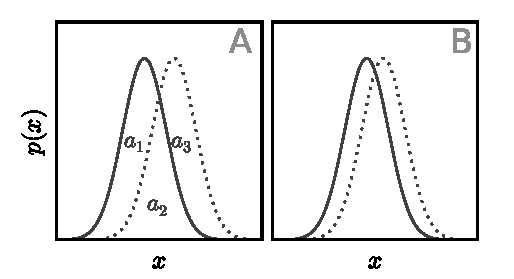
\includegraphics[scale=1.0]{figs/normal_example.pdf}
	\caption{
	  	Normal distributions exhibiting a total variational distance
		of A) 50\% and B) 30\%.  The total variational distance is 
		the non-overlapping portion of the distributions, e.g. in
		A) it is given by 
		$\theta = a_1 / (a_1 + a_2) = a_2 / (a_2 + a_3)$.
	}
	\label{fig:l1_example}
\end{figure}

Empirically measuring the divergence between distributions
is a matter of ongoing
research \cite{val-thesis,batu2013testing,chan2014optimal}.
In the ``na\"ive'' approach one first uses the samples to reconstruct 
empirical
distributions, by calculating their maximum likelihood parameters.
Then, one substitutes the empirical values of $p(x)$ and $q(x)$ into 
Equation~\ref{eq:theta} \cite{batu2013testing}.  
For example, one might directly estimate $\hat{p}(x) = N_x/N$, 
where $N_x$ is the number of times response $x$ is observed among $N$ 
total responses.

However this approach can \textit{drastically} overestimate $\theta$
\cite{val-thesis}.  As an illustrative example,
suppose that we have sampled two sets of 1000 words from \textit{possibly} 
different distributions, and that we wish to estimate the divergence 
between these distributions.  
It turns out that, if both sets of words were actually drawn from 
an identical Zipf distribution\footnote{The 
  Zipf distribution is a common model for word frequencies 
  \cite{powers1998applications,zipf1949human}:
  \begin{align}
	p(x) = \frac{x^{-1}}{\sum_{n=1}^{\infty}x^{-1}},
	\label{eq:zipf}
  \end{align}
  where $p(x)$ is the probability of the $x$th most common word.
}, the na\"ive approach would typically lead one to report 
$\hat{\theta} \approx 65\%$, event though, in reality $\theta = 0\%$
(this can be shown by simulated sampling).

However, we can establish a lower bound for $\theta$ by 
exploiting a fact about the theoretical limits on the accuracy of a 
classifier algorithm.  The intuition is as follows: 
suppose workers are shown one of two alternative designs\footnote{We will
use ``design'' in a general sense, to include both the design of the task
and of its context.  In particular, the ``design'' might include the
particular tasks that were shown beforehand, or the use of framing.}
for an otherwise
similar task, and that we build a classifier which, 
based on a worker's response, infers which of the designs had been 
used.
If worker's responses are not affected by the design alternative,
then the classification problem will be hard, and the classifier's 
accuracy poor.
Conversely, if the classifier accuracy is good, then design alternative 
must have a strong effect on the response distribution.

Stated formally, any classifier algorithm, $\mathcal{A}$, that
takes the response, $x$, of a worker, and guesses the 
design that elicited the response (from two possibilities:
$\mathrm{design}_1$ or $\mathrm{design}_2$), will do so with accuracy 
$\eta_\mathcal{A}$, that is bounded according to:
\begin{equation}
	\theta \geq 2\eta_\mathcal{A} - 1,
	\label{eq:sup:l1}
\end{equation}
where $\theta$ is the divergence between the distributions of responses
to $\mathrm{design}_1$ and $\mathrm{design}_2$.

We will now establish Inequality~\ref{eq:sup:l1} by considering an
optimal classifier having accuracy $\eta_*$.  
Let us assume that workers are shown 
$\mathrm{design}_1$ or $\mathrm{design}_2$ with equal probability.
If the worker gives the response $x$, it is optimal to guess
that the worker was shown the design most likely to elicit $x$.
In other words, if $p_i(x)$ is the probability that a worker shown 
$\mathrm{design}_i$ responds with $x$, then it is optimal to 
guess that the worker saw $\mathrm{design}_j$, where 
$j = \arg\max_j{p_j(x)}$.

Of course, neither $p_1(x)$ nor $p_2(x)$ are known.  But, on seeing $x$,
the probability that such a classifier would be correct is:
\begin{align}
  \mathrm{Pr}\{\mathrm{correct}|x\} = \frac{1}{2} 
	+ \frac{|p_0(x) - p_1(x)|}{2(p_0(x) + p_1(x))}
\end{align}
Summing over all possible responses that a worker could provide, 
$x \in \mathcal{X}$, weighted by the probability of observing $x$, 
we obtain the accuracy of the optimal classifier:
\begin{align}
\eta_* 
  &= \sum_{x\in\mathcal{X}} 
	\mathrm{Pr}\{\mathrm{correct}|x\}\mathrm{Pr}\{x\} \\
  &= \sum_{x\in\mathcal{X}} 
	\left(
	\frac{1}{2} + \frac{|p_0(x) - p_1(x)|}{2(p_0(x) + p_1(x))}
  \right) \left( 
	\frac{p_0(x) + p_1(x)}{2} 
  \right) \\
  &= \frac{1 + \theta}{2}
\end{align}
Since no classifier can be more accurate than an optimal classifier,
it follows that, for any \textit{practical classifier} 
with accuracy $\eta_\mathcal{A}$, the bound 
$\theta \geq 2\eta_\mathcal{A} -1$ holds.

Thus, we can establish a \textit{lower bound} on $\theta$ by first 
building a classifier that infers the design shown to workers from their 
responses, and then measuring its accuracy.

\section{Results}
\begin{figure}
	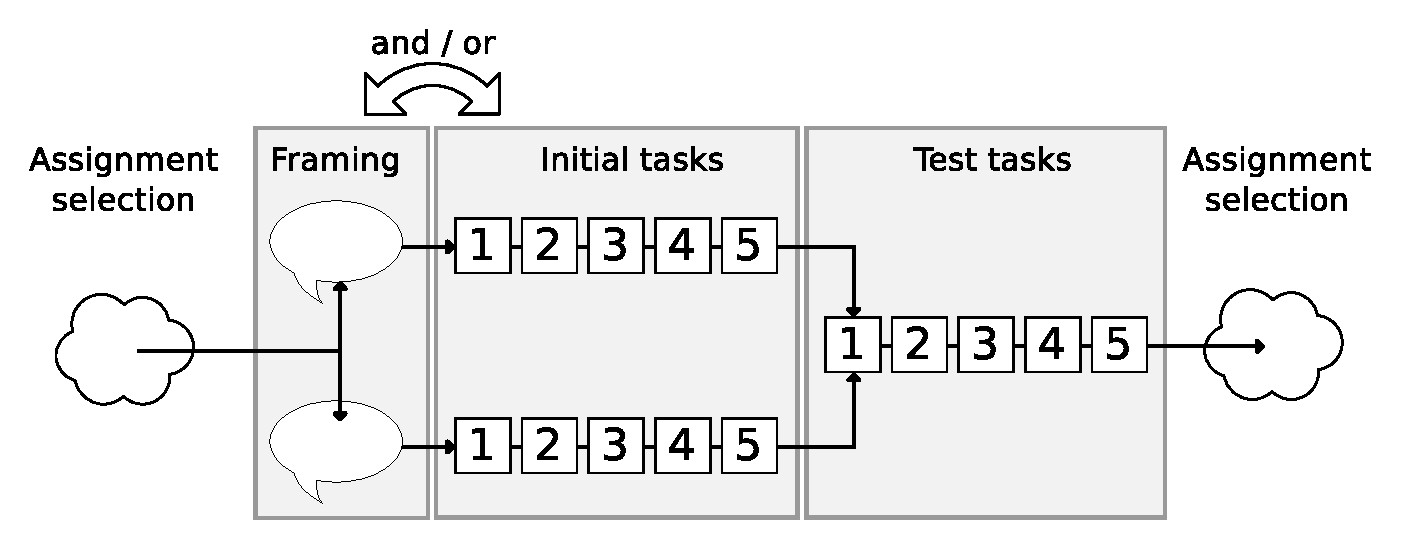
\includegraphics[scale=0.36]{figs/task-schematic-2.pdf}
	\caption{
	  Template for the experiments described in the main text.
	  After selecting our assignment on Mechanical 
	  Turk, workers were separated into two treatments.
	  Workers from each treatment were subjected to framing and/or
	  five initial tasks, which differed between treatments, and then 
	  completed a set of five test tasks that were identical for both
	  treatments.  Most experiments involved either framing or initial
	  tasks (see table \ref{table:experiments}), 
	  but \textit{frame-food-culture} involved both.
	  After the experiment, workers return to the Mechanical Turk 
	  task-selection interface.
	}
	\label{fig:task-schematic}
\end{figure}


\begin{figure*}
	\centering
	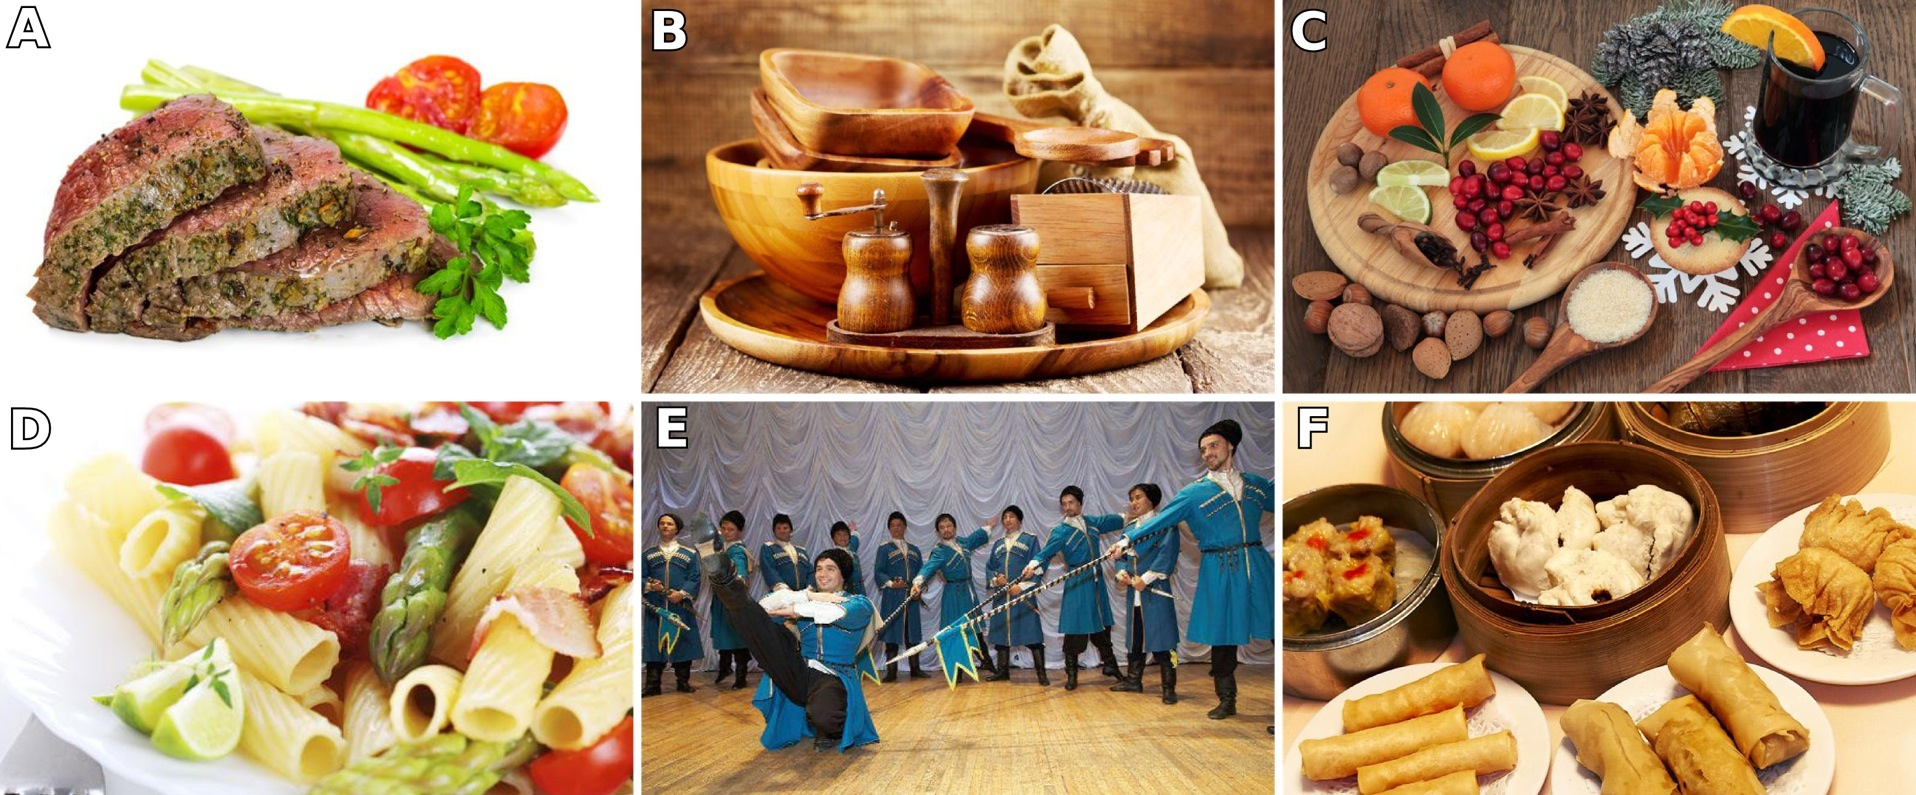
\includegraphics[scale=1.0]{figs/images.jpg}
	\caption{
		Examples of images used in
		initial tasks for the (\textbf{A}) \textit{food} and (\textbf{B}) 
		\textit{objects} treatments of \textit{intertask-food-objects};
		(\textbf{C}) test tasks for \textit{intertask-food-objects} and 
		\textit{frame-food-objects};
		initial tasks for the (\textbf{D}) \textit{food} and (\textbf{E}) 
		\textit{culture} treatments of \textit{intertask-food-culture};
		and (\textbf{F}) test tasks for \textit{intertask-food-culture} and 
		\textit{frame-food-culture}.
	}

	\label{fig:task}
\end{figure*}


\begin{figure}
	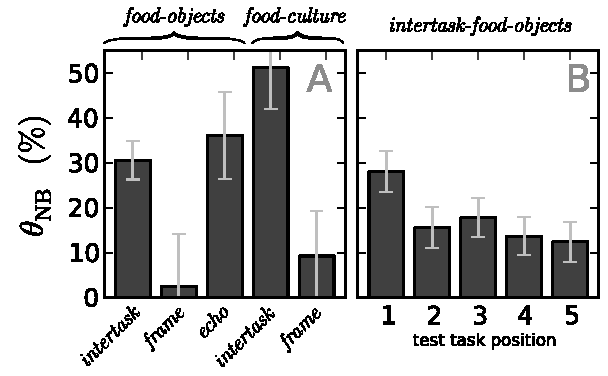
\includegraphics[scale=0.75]{figs/theta.pdf}
	\caption{
		Empirical bias, $\theta_\mathrm{NB}$, measured using a na\"ive Bayes 
		classifier, induced in image-labeling tasks, due to workers' 
		exposure to framing and prior tasks.  
		(\textbf{A}) Exposing workers to initial tasks induced more severe
		bias than framing, except when echoed framing was used. 
		(\textbf{B}) As workers proceeded through test tasks, 
		the bias due to initial tasks waned, 
		but remained significant even after five tasks.  
		Standard error bars are shown.
	}
	\label{fig:theta}
\end{figure}


\begin{table}
\small
\centering
\setlength{\tabcolsep}{1pt}
\begin{tabular}{c c c c c}
\toprule
Experiment & \parbox[c]{3.0cm}{\centering{Priming modality}} & Initial Tasks & Frame \\
\midrule
\multirow{2}{*}{\textit{intertask-food-objects}} 
& \multirow{2}{*}{initial tasks} & \textit{food} & none \\
  & & \textit{objects} & none  \\

\noalign{\smallskip}
\hdashline
\noalign{\smallskip}

\multirow{2}{*}{\textit{frame-food-objects}} 
& \multirow{2}{*}{framing} & none 
	& ``food''\textsuperscript{a} \\
& & none 
	& ``objects''\textsuperscript{b} \\

\noalign{\smallskip}
\hdashline
\noalign{\smallskip}

\multirow{2}{*}{\textit{echo-food-objects}} 
& \multirow{2}{*}{echoed framing} & none
	& ``food''\textsuperscript{c} \\
& & none & ``objects''\textsuperscript{d} \\

\noalign{\smallskip}
\hdashline
\noalign{\smallskip}

\multirow{2}{*}{\textit{intertask-food-culture}} 
& \multirow{2}{*}{initial tasks} & \textit{food} 
	& none \\
& & \textit{culture} 
	& none \\

\noalign{\smallskip}
\hdashline
\noalign{\smallskip}

\multirow{2}{*}{\textit{frame-food-culture}} 
& \multirow{2}{*}{framing} & \textit{food} 
	& ``food''\textsuperscript{e} \\
  & & \textit{food}
	& ``culture''\textsuperscript{f} \\

\bottomrule
\end{tabular}
\caption{
	Description of experiments performed.  Each experiment had two treatments
	which differed either in the initial tasks shown or the framing used 
	(the priming modality).  
	During echoed framing, the worker had to respond to the framing language
	using a combo box input.  The framing language used was as follows:
	\newline\textsuperscript{a} ``Funded by the laboratory for the visual 
		perception of Food and Ingredients''
	\newline\textsuperscript{b} ``Funded by the laboratory for the visual 
		perception of Objects and Tools''
	\newline\textsuperscript{c} ``The purpose of this study is to understand the visual perception of Food and Ingredients''
	\newline\textsuperscript{d} ``The purpose of this study is to understand the visual perception of Objects and Tools''
	\newline\textsuperscript{e} ``This research is proudly funded by The National 
		Foundation for Nutritional Awareness''
	\newline\textsuperscript{f} ``This research is proudly funded by The Global 
		Foundation for the Recognition of Cultures''
}
\label{table:experiments}
\end{table}



We performed a series of five experiments
on Amazon's Mechanical Turk\footnote{\url{mturk.com}} using 1071 workers.  
Every experiment consisted of two treatments, each with 119 workers,
who performed a single assignment\footnote{Workers could not participate 
multiple times in our study}\textsuperscript{,}\footnote{On Mechanical Turk, individual 
assignments are called Human Intelligence Tasks (HITs), but this use of 
``task'' is 
different from our current one: in our experiment each HIT actually 
involves 10 image-labeling tasks.}.  
The setup in each experiment followed the template depicted in 
Figure~\ref{fig:task-schematic}.  
The assignments had two parts.  The first part of the assignment differed
between the two treatments, and consisted of a set of initial tasks 
and/or framing (by describing the purpose of the assignment or source of 
funding).  In the second part of the assignment, workers from both
treatments completed the same five \textit{test tasks}.  Each of the 
initial and test tasks required workers to provide five descriptive labels
for an image.  The tasks were performed one at a time,
and, in treatments involving both initial and test tasks, there was no
interruption or distinction made between the initial and test tasks from
the perspective of the worker.

We analyzed the
workers' responses to the test tasks to determine whether
they were influenced by the initial tasks (or framing).  We looked for 
differences in the distributions of test responses 
using a $\chi^2$ test.  We then measured the 
severity of bias induced by initial tasks and framing, by 
constructing a na\"ive Bayes classifier to infer the workers' 
treatments based on their responses to test tasks, 
and measuring its accuracy.

In our first experiment called \textit{intertask-food-objects},
workers were assigned to either a \textit{food} or \textit{objects} 
treatment.  Workers from these treatments performed initial tasks 
in which they labeled, respectively, 
images depicting either food or (non-food) objects
(see example images in Figure~\ref{fig:task}A and B).  
Workers from both treatments then performed five test tasks, which
contained images
depicting both food and objects (Figure~\ref{fig:task}C).  

The frequencies of words used by
workers in the \textit{food} and \textit{objects} treatments differed
significantly during test tasks (by $\chi^2$ test, $p = 6.0 \times 10^{-14}$),
even though the test tasks were identical in both treatments.  
Thus earlier tasks do significantly affect later ones, which 
validates our concerns about the typical microtask methodology.

Having affirmed the \textit{existence} of intertask effects, we sought to
measure the severity of the bias induced, i.e. $\theta$.
To measure $\theta$ we used a na\"ive Bayes classifier based on a 
multinomial distribution over the word frequencies in worker's labels, 
and measured it's accuracy using leave-one-out cross-validation.  
We chose the na\"ive Bayes
classifier for three reasons.  First, it performs well even when the 
number of features is large compared to the number of training examples.  
Second, there are no hyperparameters to 
optimize, which eliminates the need to partition the response data into
dev and test sets.
Third, the conditional independence assumption, normally 
undertaken for pragmatic reasons, is probably a relatively mild in 
relation to image labels, since they are likely to be less dependent
on one another than in a coherent passage of text.  We also used a 
support vector machine and found very similar results.

To produce word frequency features, worker's labels were split on white
space and punctuation, and the resulting tokens were spell-corrected based
on edit-distance to a dictionary of words, followed by stop-word removal
and lemmatization.  The spelling correction
dictionary was compiled from a combination of WordNet 
\cite{felbaum1998wordnet} and words
collected by crawling the World Food section of \url{allrecipes.com}.

Based on the classifier accuracy, intertask effects in the 
experiment \textit{intertask-food-objects}
lead to (a lower bound) bias of $\theta=30\%$ between workers from the 
\textit{food} and \textit{objects} treatments (Figure~\ref{fig:theta}A).
It is difficult to visualize the distributions of word frequencies,
but for reference, the distributions shown in 
Figure~\ref{fig:l1_example}B have $\theta = 30\%$.  This represents a 
substantial potential to distort microtask data.

As already discussed, there has been considerable interest in the 
effects that framing can have on microtask responses
\cite{Kinnaird2012281,chandler2013breaking,thibodeau2013natural}, and 
framing effects are arguably similar to inter-task effects in the sense 
that both arise from the worker's experiences immediately before 
performing a task.
Therefore, as a point of comparison, we performed a similar experiment 
in which we suggested the focus of the study by stating a name for
the requester within the task.
In the experiment 
\textit{frame-food-objects}, we used the same test tasks as in 
\textit{intertask-food-objects}, but the initial tasks were omitted, 
and in their stead, workers were either told that the study was 
``Funded by the laboratory for the 
visual perception of Food and Ingredients'', 
or ``\ldots of Objects and Tools''.  

Framing induced changes in the frequencies of 
word usage at significance 
(as determined by $\chi^2$ test; $p=0.0012$).  But, 
the \textit{extent} of framing-induced bias was not statistically 
distinguishable from zero ($p =0.37$) (Figure~\ref{fig:theta}A).
And so, remarkably, the extent of bias due to framing was weaker than that 
due to intertask effects ($p=2.1\times 10^{-5}$).
In other words, the \textit{microtasks themselves}
had a stronger biasing effect than framing.

To assess the persistence of intertask effects, we replicated the 
\textit{intertask-food-objects} experiments, rotating the ordering of the
test tasks, so that each test task occupied each of the possible 5 
test-task positions (see Figure \ref{fig:task-schematic}).  
By taking the average bias induced for each test task when 
occupying a given position, we determined $\theta$ as a function of the 
task position.
Bias was strongest for the first test task (about 28\%), 
but remained significant through all five test tasks 
($\alpha=0.05$) sustaining over 12\% bias even when the initial and test 
tasks were separated by four intervening tasks (Figure~\ref{fig:theta}B).

We conducted variants of these experiments using different images, to see 
whether this trend was robust.  In the experiment 
\textit{intertask-food-culture},
workers were either assigned to a \textit{food} or \textit{culture} treatment.
The initial tasks contained either images 
depicting food (Figure~\ref{fig:task}D), or depictions of cultural scenes 
(of dance, sport, or music) (Figure~\ref{fig:task}E).  The test tasks, 
which 
were, again, identical for both treatments, depicted meals of diverse 
cultural origin
%\footnote{
%  	The food depicted in the initial tasks 
%	in \textit{intertask-food-culture} are arguably still of
%	diverse cultural origin, but this would only tend to make our 
%	results more conservative.
%}
(Figure~\ref{fig:task}F).  

Results for this experiment again showed a 
strong bias as a result of intertask effects (about 50\%) 
(Figure~\ref{fig:theta}A).  Again, visualizing the word frequencies 
themselves is difficult, but Figure~\ref{fig:l1_example} provides an 
example of distributions having $\theta = 50\%$.

Once again, we compared the strength of intertask effects to those due to 
framing. In the experiment \textit{frame-food-culture} we used
the same test tasks as in \textit{intertask-food-culture}, but before
workers began the tasks, we indicated
that the purpose of the task was either the recognition of food or 
culture, depending on the treatment to which the worker was assigned.  
However, unlike in the previous framing experiment, this time we also 
included initial tasks in the framing experiment (although they were 
identical for both treatments).  We did this in order to include a pair of
comparable priming- and framing-based experiments
for which both had the same overall number of tasks.
In \textit{frame-food-culture}, framing did not induce 
significant changes in word frequencies 
(by $\chi^2$ test, $p=0.29$) (Figure~\ref{fig:theta}A).

It was only when framing was combined with an active reiteration step, 
that framing-induced bias reached a comparable extent to that induced by 
intertask effects.  In the experiment \textit{echo-food-objects},
after framing the purpose of the task (as the recognition of food
or objects), workers were asked to echo the purpose of the task
using a combo-box input.  This  ``echoed framing'' induced a bias of about 
35\% (Figure~\ref{fig:theta}A). However, it is difficult to say whether this 
should be considered as a framing treatment \textit{per se}:
requiring the worker to reiterate the purpose signals our intent, as the 
requester, to ensure that the worker has taken note of it, possibly leading 
the worker to interpret the exchange as an instruction.  
In any case, it is remarkable that intertask effects
were on par with an explicit, actively reinforced statement of the tasks' 
purpose.

\begin{figure}
	\centering
	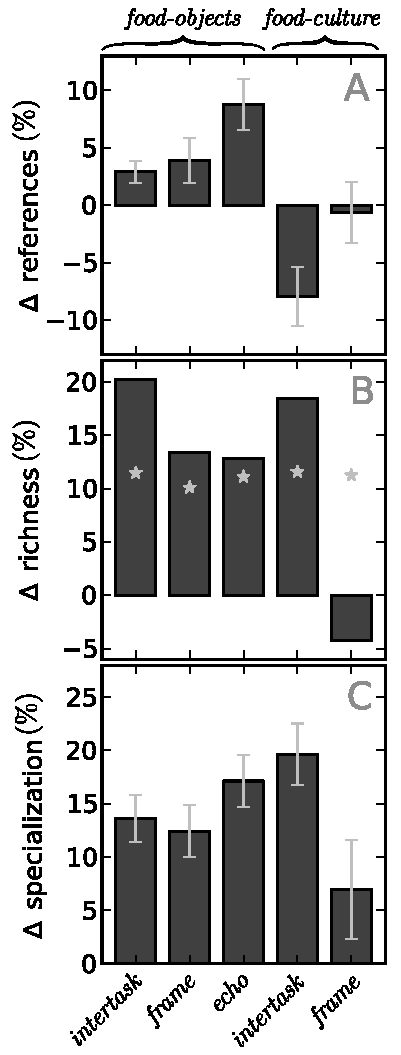
\includegraphics[scale=0.87]{figs/vocab_specificity.pdf}
	\caption{
		Exposing workers to a priming concept, e.g. food, through
		initial tasks or framing, affects their tendency to focus
		on that concept, and the richness and specialization of their 
		vocabulary in reference to it.
		In all three plots, positive values indicate a larger quantity for 
		the food-exposed workers.
		(\textbf{A}) Exposing workers to food does not necessarily increase
		the fraction food references they provide during test tasks.
		(\textbf{B}) The number of unique food-related
		words (richness) was greater for food-exposed workers, except in the 
		case of \textit{frame-food-culture} (stars indicate the threshold
		for a significant deviation, $\alpha=0.05$). 
		(\textbf{C}) Food-exposed
		workers used more specialized words to refer to food.
		Standard error bars are shown in (\textbf{A} and \textbf{C}).
	}
	\label{fig:specificity}
\end{figure}

\begin{table*}
	\centering
	\setlength{\tabcolsep}{4pt}
	\begin{tabular}{ c c c c c }
	
		\setlength{\tabcolsep}{4pt}
		\begin{tabular}{ r | c }
		\toprule
		\multicolumn{2}{c}{
			\parbox[c]{2.5cm}{
				\centering
					\textit{intertask-food-objects}
			}} \\
		\midrule
		coffee & 38 \\
		meal & 34 \\
		cheese & 34 \\
		apple & 32 \\
		dessert & 21 \\
		cup & -30 \\
		glass & -45 \\
		table & -70 \\
		candle & -74 \\
		food & -80 \\
		\bottomrule
		\end{tabular}

&

		\setlength{\tabcolsep}{4pt}
		\begin{tabular}{ r | c }
		\toprule
		\multicolumn{2}{c}{
			\parbox[c]{2.5cm}{
				\centering
				\textit{frame-food-objects}
			}
		}\\
		\midrule
		bread & 18 \\
		wine & 18 \\
		cheese & 16 \\
		apple & 14 \\
		oil & 12 \\
		table & -9 \\
		meal & -10 \\
		candle & -12 \\
		dinner & -13 \\
		food & -32 \\
		\bottomrule
		\end{tabular}

&

		\setlength{\tabcolsep}{4pt}
		\begin{tabular}{ r | c }
		\toprule
		\multicolumn{2}{c}{
			\parbox[c]{2.5cm}{
				\centering
			\textit{echo-food-objects}} 
		}\\
		\midrule
		apple & 24 \\
		cheese & 23 \\
		wine & 15 \\
		coffee & 14 \\
		oil & 7 \\
		knife & -24 \\
		dinner & -26 \\
		fork & -27 \\
		candle & -35 \\
		food & -55 \\
		\bottomrule
		\end{tabular}

&

		\setlength{\tabcolsep}{4pt}
		\begin{tabular}{ r | c }
		\toprule
		\multicolumn{2}{c}{
			\parbox[c]{2.5cm}{
				\centering
			\textit{intertask-food-culture}} 
		}\\
		\midrule
		spicy & 26 \\
		sauce & 17 \\
		indian & 15 \\
		buffet & 14 \\
		exotic & 12 \\
		festival & -11 \\
		offering & -12 \\
		statue & -15 \\
		india & -20 \\
		food & -56 \\
		\bottomrule
		\end{tabular}

&

		\setlength{\tabcolsep}{4pt}
		\begin{tabular}{ r | c }
		\toprule
		\multicolumn{2}{c}{
			\parbox[c]{2.5cm}{
				\centering
			\textit{frame-food-culture}} 
		}\\
		\noalign{\smallskip}
		\midrule
		indian & 11 \\
		banquet & 8 \\
		spicy & 7 \\
		asian & 6 \\
		variety & 6 \\
		delicious & -6 \\
		meat & -7 \\
		festival & -7 \\
		spice & -7 \\
		food & -9 \\
		\bottomrule
		\end{tabular}

	\end{tabular}
	\caption{
		The five words whose frequencies increased, and those whose 
		frequencies decreased, the most, between treatments of given 
		experiments, within labels attributed to the first test task.
		Values indicate the absolute change in number of occurrences
		of the word, and positive values indicate that the food-exposed
		treatment 
		used the word with higher frequency.  
		Note that the word ``food'' is always the most suppressed among
		food-exposed workers.
		Word frequencies for 
		\textit{intertask-food-objects} correspond to the labels attributed
		to image 1 which is not necessarily the first 
		test task due to the tasks being permuted.  There were five times
		as many workers in \textit{intertask-food-objects}, hence
		larger absolute differences are observed.
	}
	\label{table:top-words}
\end{table*}

To better understand the nature of 
intertask effects, we investigated the vocabulary
that workers used to label test tasks. One might expect that, within a given 
experiment, those workers exposed to food (whether through framing or initial
tasks) would label test tasks using 
food-related words more often.  To test this we developed an 
automated approach to labeling food-words based on the 
WordNet knowledge base \cite{felbaum1998wordnet}.  

WordNet provides
hyponym and hypernym relations between words.  A hypernym is a 
generalization (for example, ``bread'' is a hypernym of ``pumpernickel''), 
while a hyponym is a specialization.  We took took the set of food-words
to be all those reachable through
a chain of hyponym relations from the word senses 
\texttt{food.n.01} and \texttt{food.n.02}, in other words, all words
denoting a specific kind of food (a total of 3590 words).  
To improve the coverage of words for
less widespread foods, we augmented this set with all words
discovered while crawling the World Food section of \url{allrecipes.com} 
which were not already in WordNet.  

To validate the resulting set of 
food words, three independent annotators labeled 500 words selected from 
workers' responses as either food or non-food, and these were
compared to the labels derived using the automated approach.
Among those words, 26\% were 
deemed to be food by the majority of annotators.  
Taking the majority label among annotators to be the correct one, 
the automatically-identified food-words
had 88\% correspondence to the human annotators.  Treating the
automated identification of food words as another annotator, there 
was an inter-rater reliability of 82.4\%.

Using the automated labeling of food words, we found that, in fact
workers exposed to food (via prior tasks or framing) did not necessarily
use more food-words when labeling images in the test tasks.
In \textit{intertask-food-culture}, food-exposed
workers actually used significantly \textit{fewer} food-related words 
during test tasks (Figure~\ref{fig:specificity}A).  This finding
rules out a seemingly-simple idea that workers emphasize
content that has been present in earlier tasks: seeing content 
influences, but does not necessarily \textit{increase}, the probability of 
referring to it in subsequent tasks.

To deepen our understanding, we investigated workers' lexical richness in 
reference to food, that is, the number of \textit{unique} food-related words
used.  Even if workers provide an abundance of food-related words, there
can be less diversity, if, for example, workers repeat generic references 
to food.
Both \textit{intertask} experiments showed that food-exposed workers had 
greater lexical richness, in reference to food, than their counterparts 
(as much as 20\% more) (Figure~\ref{fig:specificity}B).  
This is particularly noteworthy in the experiment
\textit{intertask-food-culture}, because there,
food-primed workers made fewer total references to food.  
%We also observed enrichment of the food-related lexicon in the 
%\textit{priming-food-objects}, and \textit{echo-food-objects} experiments, 
%although to a lesser extent.

The observations regarding lexical richness suggest that 
initial tasks might influence workers to use more refined or specialized 
words, when referring to aspects of content that had been present in the 
initial tasks.  
To test this, we used the hypernym and hyponym relations in WordNet 
to operationalize the notion of word specialization.  
Within each experiment, we determined relative specificity
of the food-words, between the treatments using the following equation:
\begin{equation}
	S(P,Q) = \frac{
		\sum_{w\in P}\sum_{v\in Q} \left(
			\mathbf{1}_{[w>v]} - \mathbf{1}_{[v>w]} \right)
	}{
		\sum_{w\in P}\sum_{v\in Q} \left(
			\mathbf{1}_{[w>v]} + \mathbf{1}_{[v>w]} \right)
	},
\end{equation}
where $P$ and $Q$ are sets of words associated to different experimental 
treatments, and $\mathbf{1}_{[w>v]}$ evaluates
to 1 if synset $w$ is more specific than (i.e. is a hyponym of) synset $v$.
The relative specificity lies within $[-1,1]$; 
we report it as a percentage.
In computing this quantity between two treatments, we first computed the 
relative specificity for the treatments separately for each test task, and 
averaged the results obtained across the five test tasks.

In all experiments except \textit{frame-food-culture}, food-primed workers 
used significantly more specialized words, in reference to food 
(about 15\% more) (Figure~\ref{fig:specificity}C).
It is interesting that such substantial increases in both the lexical 
richness and specialization of food-related words 
held for \textit{intertask-food-culture}, where, as mentioned, we observed 
that food-exposed workers made \textit{fewer} references to food overall. 
These observations point 
to countervailing factors: one factor tending to activate the more 
specialized and less common food-related words 
(yielding greater lexical richness and specialization), and the other tending 
to suppress certain, presumably more common and generic words 
(yielding fewer food-related words in total).

This hypothesis is corroborated when we look at those words whose 
frequencies changed the most from one treatment to another 
(Table~\ref{table:top-words}).  
The word ``food'', which is the most generic possible food-related word, was 
always \textit{suppressed} among food-primed workers.  In fact, 
for all experiments, ``food'' was the \textit{most suppressed} word.

\section{Discussion}
Our results can be 
explained through a combination of positive and negative priming.
Positive priming (usually simply ``priming'') occurs when a prior stimulus 
predisposes a person to give certain responses in an ensuing task, and
is often observed as an increase in the speed or accuracy of a response, or
the ability to recognize briefer or noisier stimuli 
\cite{BJOP1796,BJOP1826,Huber2008324}.
Negative priming occurs when, after exposure to a stimulus 
considered to be non-salient, subsequent recognition of the stimulus is 
inhibited \cite{mayr2007negative}.

Workers exposed to images containing food are (positively) primed, 
activating memories, concepts, and vocabulary related to food.  
However, if the worker labels several images containing food, the basic 
fact that an image contains food will not seem salient, since it 
does not distinguish one image from another.  Thus, the most 
generic references to that fact, such as the label ``food'', 
will be suppressed, while more specialized references will be elicited.  
Meanwhile, the number of references to food overall might increase or 
decrease, depending on the balance of these factors.  

More generally, we are suggesting that, even though workers are not 
instructed to compare tasks in any way, prior tasks form a 
context relative to which workers judge salience.  Thus, due to a combination 
of negative and positive priming, a worker's focus 
in repeated tasks tends to be directed away from generic, shared features, 
toward specific and distinguishing ones.

Prior to this study, little thought appears to have been given to
earlier tasks as a priming vector for later tasks.
But our findings show this is an important design consideration.  
One recourse might be to randomize task ordering, a practice that is 
commonly employed.  But the sheer extent of bias we observed suggests that 
this will still admit a significant amount of noise.  
Even chains of two or three similar tasks, which
will not be reliably eliminated in random permutations, could lead
to the levels of bias we observed in our experiments.
Preferably, a deeper understanding of intertask effects might allow them
to be properly controlled.

Our findings also suggest that careful task engineering might leverage
intertask effects to achieve greater quality and reproducibility in 
crowdsourcing.
A consistent goal in human computation is the achievement of expert-level
judgments from non-expert workers \cite{kittur2011crowdforge}.  
This has been achieved in some
applications \cite{snow2008cheap,Mortensen20131020,Warby2014385}. 
The distinction between experts and novices is partly attributable
to specialized knowledge and heuristics. 
But experts also simplify tasks by more efficiently directing 
their focus toward salient features \cite{kellman2009perceptual}.  
Using strategic task exposure during training, 
it might be possible to guide workers' focus 
and salience attribution, enabling expert-level 
judgment in a wider variety of
crowdsourced applications.
We anticipate future work will yield techniques to control intertask 
effects, to reduce unwanted bias, and to tune the focus, diversity, and 
specificity of worker responses.

We have shown that a severe bias can be introduced into microtask 
responses, simply from the performance of earlier tasks. 
These effects are much stronger than those of framing.  
While our findings raise serious concerns about the 
current state of microtask design, they reveal potential opportunities 
to refine worker focus and acuity.  Any application that relies
on the repetitive use of human judgment is likely subject to the phenomena
described here.  Exploring the pitfalls and opportunities posed by
intertask effects is an important direction for future work, 
in the effort to develop performant and reliable human computation.

\bibliographystyle{SIGCHI-Reference-Format}
\bibliography{newbib}

\end{document}

%%% Local Variables:
%%% mode: latex
%%% TeX-master: t
%%% End:
